\section{Literature Review}

\subsection{Motor-sport Aerodynamics}
In 1949 Ludwig Prandtl stated, "The term aerodynamics is generally used for the problem arising from a flight and other topics involving the flow of air \cite{Anderson2010FundamentalsAerodynamics}". By definition, Aerodynamics is one of the branches in physics which concern and study the interaction of a body and fluid flow stream \cite{Scibor-Rylski1984RoadAerodynamics}. The forces' magnitude and direction that occur on a body is the result of flow interaction which depends on several geometric variables. Some fundamental variables in aerodynamics include flow velocity, temperature, pressure, and density, further describing the flow physics and characteristic. Drag and lift are the most significant consideration in race-car aerodynamics, which will be discussed further in this paper's following subsection.

\noindent Aerodynamics is generally classified into external (flow around the body) and internal (flow inside the body). This paper will focus on external aerodynamics, which focuses on force generation due to the air-stream behaviour around the body of interest. In the automotive industry, external force plays an integral part since the car's overall performance depends on the aerodynamics forces created, significantly influencing and improving the vehicle shape to its aerodynamics advantage \cite{Scibor-Rylski1984RoadAerodynamics}. Some aerodynamics consideration to a vehicle's shape influence includes; large downforce generation and balance between front and rear tyre, and drag minimisation. Table \ref{Table1} shows the effect of downforce on a racing car's acceleration; it can be seen that downforce significantly improves the acceleration time by -1.06 seconds, rate of acceleration by 4.5 $m/s^2$, and power by 124 kilowatts. 

\begin{table}[!ht]
\caption{\label{Table1} Aerodynamic downforce effect of a racing car acceleration \cite{Scibor-Rylski1984RoadAerodynamics}.}
\vspace{-5mm}
\begin{center}
 \begin{tabular}{||c| c| c ||} 
 \hline
 Variables & With Downforce & Without Downforce \\ [0.5ex] 
 \hline\hline
 Time from 0 to 160 $km/h$ & 5s & 6.06s \\ 
 \hline
 Rate of acceleration at 44 $m/s$ & 10.02 $m/s^{2}$ & 5.52 $m/s^2$ \\
 \hline
 Power transferred at 44 $m/s^2$ & 353 kW & 229 kW  \\
 \hline
\end{tabular}
\end{center}
\end{table}

\noindent Queen's Formula Racing has started to focus on aerodynamics since 2016. Previous students have attempted to analyse the previous QFR car, including the undertray to optimise its overall performance.  This paper will solely focus on external aerodynamics to understand QFR undertray's flow behaviour and its force generation, which the analyses then are used as geometry consideration of the final aerodynamic undertray design.

\subsection{Aerodynamics Fundamental}
To fully understand the flow physics and behaviour of the aerodynamic undertray, there are several fundamental understanding or terminologies of aerodynamics which needs to be firstly understood.

\subsubsection{Flow Types}
The main characteristic of a liquid is the molecule ability to move around the space freely. The liquid molecule movement to another point in space also requires energy, mass, and momentum to be transferred with it. On this occasion, a "transfer phenomena" occurred, where the molecules introduced to viscosity (friction), thermal conduction, and mass diffusion \cite{Anderson2010FundamentalsAerodynamics}. The flow that shows the indication of "transfer phenomena" can be called viscous flow. On the other hand, the flow condition where the "transfer phenomena" does not occur is known as inviscid flow.

\noindent Some flow such as streamline far from the wall can be represented by the inviscid flow. But to capture the aerodynamic behaviour between two walls, such as an undertray, the viscous flow plays a crucial factor. The shear stress near wall boundaries occurs due to the viscosity, which becomes one of the significant drag sources. The presence of viscosity allows the simulation to capture flow separation on the high incident geometries. The viscous effect is an essential consideration in the analysis where the body of interest is purposely designed to generate aerodynamic forces due to the flow, such as airfoil and undertray.

\noindent Another vital property in aerodynamics is density ($\rho$). Compressibility on a flow is entirely dependant on the state of its density at a certain speed. Incompressible flow can be referred to as a flow with constant density throughout, which usually happens at Mach number less than 0.3. In contrast, the region of Mach greater than 0.3 is known as compressible flow, where density varies \cite{Anderson2010FundamentalsAerodynamics}.

\subsubsection{Reynolds Number}
Reynolds number is a dimensionless ratio of inertial and viscous forces used to classify the probability of flow being laminar or turbulent\cite{Rehm2008SituationalMPD}. Mathematically, Reynolds Number can be expressed as:

\begin{equation}
Re = \frac{\rho v d}{\mu} = \frac{inertial force}{viscous force}
\end{equation}

\noindent For low Reynolds number, the flow can be categorised as laminar where the molecules move in a regular, smooth, steady, and no mixing between layer occurred\cite{Obidi2014TheoryVehicles}. In contrast, the turbulent flow usually occurs at a high Reynolds number where the fluid particles travel in a random and irregular attitude that breaks up the streamline. When the flow is changing from laminar to turbulent, this flow is called the transition region. Figure \ref{fig:2} shows the difference in laminar flow with a transition to the turbulent region near the wall. 

\begin{figure}[!htb]
    \centering
    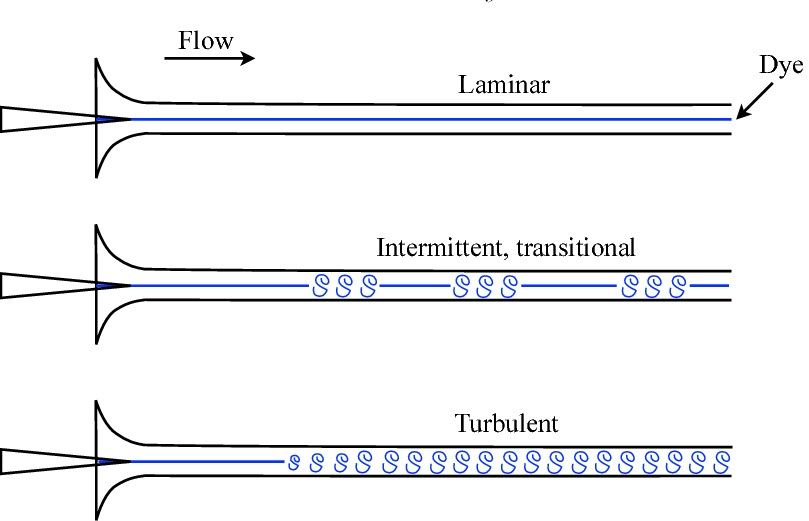
\includegraphics[scale=0.4]{Figures/laminar_turbulent_difference.jpg}
    \caption{Illustration of difference between laminar, transition, and turbulent flow in a pipe \cite{D.BARKLE2016TheoreticalPipe}.}
    \label{fig:2}
\end{figure}

\subsubsection{Boundary Layer}
The boundary layer is referred to as the viscous flow region adjacent to the body surface \cite{Anderson2010FundamentalsAerodynamics}. The layer of air stream surrounding the body at a distance near the wall moves with various relative speed; therefore, this creates a velocity gradient ($\frac{\partial V}{\partial y}$) which the speed on the surface is zero (non-slip condition) to local velocity outside the surface layer \cite{Scibor-Rylski1984RoadAerodynamics}. This layer is also referred to as a boundary layer. Figure \ref{fig:3} shows the development of a boundary layer on a flat plate; it started with laminar flow, which transitioned into turbulent flow with the formation of eddies.

\begin{figure}[!htb]
    \centering
    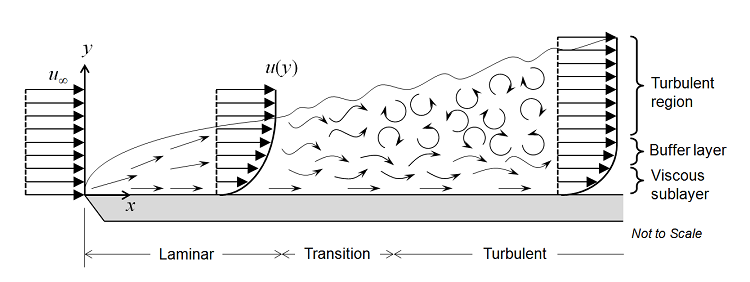
\includegraphics[scale=0.6]{Figures/BL_laminar_turbulent.png}
    \caption{The difference of boundary layer along flat plat \cite{Frei2017WhichApplication}.}
    \label{fig:3}
\end{figure}

 
\noindent From figure \ref{fig:3}, it can be seen that there are two main types of boundary layer flow: laminar and turbulent. Laminar is demonstrated close to the leading edge where the fluid travel smoothly, which shows a low-velocity gradient and low friction near the wall. When the velocity gradient increases and the friction on one layer to another are significant, this flow can be stated as turbulent \cite{Scibor-Rylski1984RoadAerodynamics}. Turbulent flow can be indicated as an irregular and random fluid movement with the presence of eddies. The boundary layer is essential due to its ability in producing drag due to skin friction. When the local velocity increases, the velocity gradient $(\frac{\partial V}{\partial y})_{y=0} $ and shear stress near the wall ($\tau_w $) also increases with the overall drag.

\noindent It has to be noted that turbulent flow and separated flow are related but different flow characteristic. Flow separation occurs where the air stream effect is reversed when the surface geometry is curving away. When the air stream slows down, the pressure gradient inverses, which create an adverse pressure gradient and then cause a thickening in the boundary layer \cite{Scibor-Rylski1984RoadAerodynamics}. The condition let the shear stress (friction) and adverse pressure gradient bring the molecules near the wall to stop. At this stage, the boundary layer separates and create a region of reversed flow. This condition is illustrated on figure \ref{fig:flow separation}.

\begin{figure}[!ht]
    \centering
    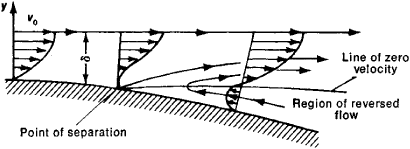
\includegraphics[scale= 0.8]{Figures/flow_separation.png}
    \caption{Illustration of separated flow formation along curved body \cite{Anonymous1979SeparationDictionary}}
    \label{fig:flow separation}
\end{figure}

\subsubsection{Bernoulli Equation \& Venturi Effect}
Bernoulli equation is another critical mathematical analysis that analyses the relationship between flow speed and pressure; this is a fundamental aerodynamic undertray theory. The equation can be expressed as:
\begin{equation}
   \underbrace{p}_\textrm{Pressure Energy} + \underbrace{\frac{1}{2} \rho V^{2}}_{\substack{\text{Kinetic Energy} \\ \text{per Unit Volume}}} + \underbrace{\rho g h}_{\substack{\text{Potential Energy} \\ \text{per Unit Volume}}} = constant
    \label{eq:bernoulli}
\end{equation}

Equation \ref{eq:bernoulli} clearly states the relationship between speed and pressure where the flow's density is assumed constant. The equation states that pressure is inversely proportional to the airspeed; therefore, an increase in velocity has to be accompanied by a reduction in pressure and vice versa. This strongly correlated to the downforce generation of an undertray, flow acceleration on the bottom of a car will reduce the pressure, hence high downforce.

\noindent The underbody of a race car can be modelled as a Venturi tunnel where the undertray the airflow goes into area convergence then expanded at the rear, illustrated in figure \ref{fig:venturi_tunnel_car}. This shape aims to promote the venturi effect in the proximity of the ground, which increases the downforce and reduces drag \cite{Katz2005AerodynamicsCars}. The continuity formula $\rho AV = constant$ stated the reduction in underbody cross-sectional area increases the velocity, hence decreases the pressure (from equation \ref{eq:bernoulli}).

\begin{figure}[!ht]
    \centering
    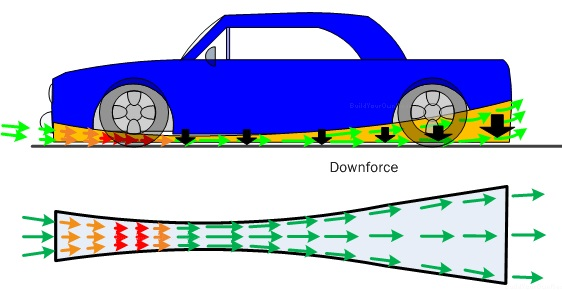
\includegraphics[scale=0.8]{Figures/venturi_tunnel.jpg}
    \caption{Venturi tunnel modelling of an automotive underbody \cite{Anonymous2020RaceDesign}.}
    \label{fig:venturi_tunnel_car}
\end{figure}

\noindent It is worth to be noted that this simplification only applied in an ideal condition where the air mass is fully conserved throughout the undertray. In real-life conditions, there are some air leakages on the side of the undertray and create corner vortices that significantly affect overall car performance. The rule of thumb for designers is to maximise the cross-sectional area reduction on the inlet and area expansion on the rear; this case will not be possible due to viscosity. High area reduction on the inlet will accelerate the flow and proportional to drag increase, and high diffuser area (outlet angle) will create flow separation, which reduces the downforce and creates a significant wake at the rear of the car hence higher drag. To achieve an optimised underbody design, broad variables must be widely and deeply analysed to identify their effect on the aerodynamic force.


\subsubsection{Aerodynamic Forces}
Forces optimisation generated by the aerodynamic flow is the main goal of this paper. The Bernoulli Equation from section 2.2.4 indicated that the flow pattern around a body produces pressure distribution over the surface \cite{Scibor-Rylski1984RoadAerodynamics}, which means integrating the pressure over the body surface will result in total forces caused by the flow around the body. The general force equation of a body can be expressed as:
\begin{equation}
    F = qSC_f
\end{equation}
Where $C_f$ is a dimensionless coefficient dependent on the body's shape \cite{Scibor-Rylski1984RoadAerodynamics} and $S$ is the area on which the surface the force of a body. In a drag analysis, the surface is the frontal area of a body that imposed the flow velocity (illustrated on figure \ref{fig:Force direction and frontal area} right). On the other hand, the lift analysis will require the area of the lift generator (e.g. undertray, inverted wing, or car wetted-surface).

\begin{figure}[!h]
\begin{center}
%    
  \begin{subfigure}[b]{0.4\textwidth}
    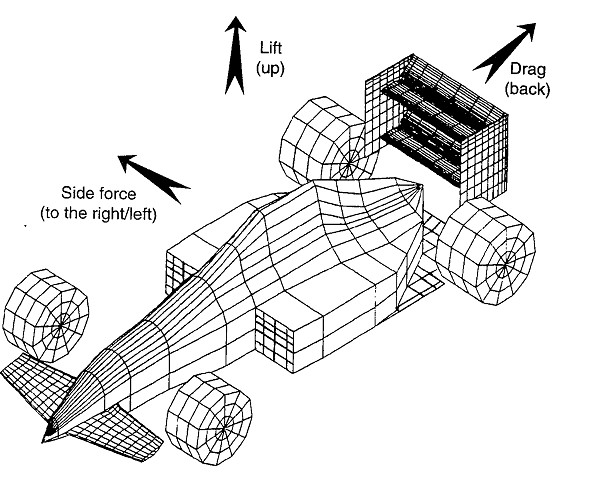
\includegraphics[scale=0.4]{Figures/race_car_forces.jpg}
  \end{subfigure}
  %
  \begin{subfigure}[b]{0.4\textwidth}
    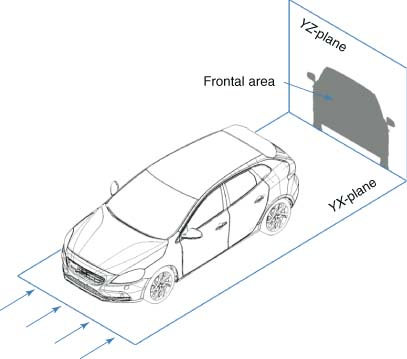
\includegraphics[scale=0.8]{Figures/frontal_area.jpg}
  \end{subfigure}
%  
  \caption{Force direction acting on a race-car(left) and representation of frontal area of an automotive body(right)\cite{Sebben2014FundamentalsDesign}.}
    \label{fig:Force direction and frontal area}
\end{center}
\end{figure}
\noindent There are three main forces acting on a car body: lift, drag, and side force. Figure \ref{fig:Force direction and frontal area} left illustrate the direction of forces acting on a car. Due to the function of undertray, this paper will only focus on the generation and optimisation of lift and drag.

\paragraph{Lift (downforce)}
Lift is an applied force due to the pressure difference on a body, which acts vertically and perpendicular to the drag force \cite{Scibor-Rylski1984RoadAerodynamics}. Lift can be mathematically expressed as:
\begin{equation}
    L = \frac{1}{2}\rho U^2 S C_L
\end{equation}
It is important in the motor-sport industry that a race car produces as much downforce (negative lift) with the least drag possible. In the aviation field, the aerofoil generates positive force to lift the aircraft from the ground; on the other hand, lift on race car used to increase the tyre grip by using an inverse aerofoil concept which produces a negative force. This consideration is due to the significant improvement in road handling and tyre grip, enabling higher cornering speed, acceleration, and braking \cite{Barnard1997RoadIntroduction}.


\paragraph{Drag}
Drag is a force that works against the intended direction of a body, which manifests in friction or pressure \cite{Obidi2014TheoryVehicles}. The drag force direction always follows the flow velocity of the car motions. Drag force can be mathematically expressed as:
\begin{equation}
    D = \frac{1}{2}\rho U^2 S C_D
\end{equation}
In a formula student car, the flow that travels around the car can be assumed as stokes flow (low Reynold number flow) which stated that drag is directly proportional to the viscosity, velocity, and size \cite{Obidi2014TheoryVehicles}. If the viscosity of air can be assumed as constant in the analysis, the only variable that could be modified to reduce the drag is the body's size or geometry. It has to be noted that race-car drag also divided into five different types of drag \cite{Kelly1964AerodynamicsEngineers}: form drag, lift drag, surface drag, interference drag, internal flow drag.

\subsection{Aerodynamics Undertray}
Undertray is an aerodynamics device that is attached to the underside of a race car that take advantages of the aerodynamic flow to decreases the pressure and increase the downforce significantly. Undertray has become an important part in motor-sport industry due to its ability to produce 45\% of car's downforce \cite{Katz1995RaceSpeed}. A typical undertray consist of a nozzle (inlet), floor section (throat), and diffuser (outlet).  Figure \ref{fig:underbody} shows an example of simple undertray of a formula car.

\begin{figure}[!ht]
\begin{center}
%    
  \begin{subfigure}[b]{0.4\textwidth}
    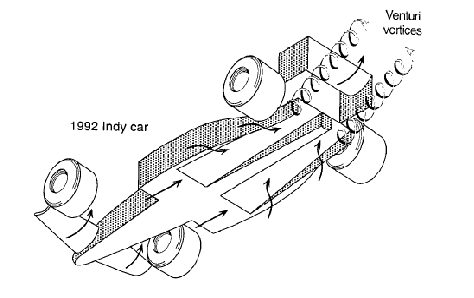
\includegraphics[height=4.8cm]{Figures/underbody.PNG}
  \end{subfigure}
  %
  \begin{subfigure}[b]{0.4\textwidth}
    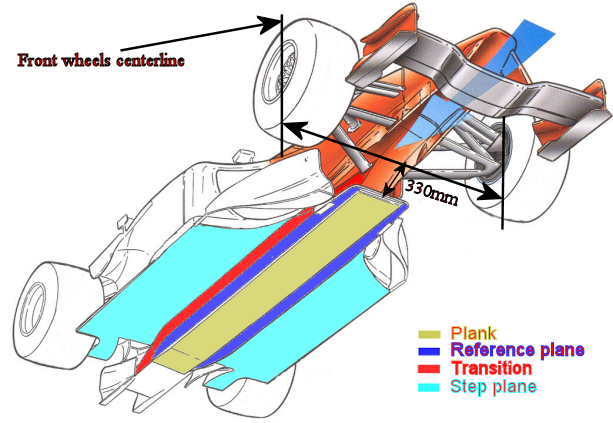
\includegraphics[height=4.8cm]{Figures/undertray_f1.png}
  \end{subfigure}
%  
  \caption{Typical undertray of a formula race-car \cite{Katz1995RaceSpeed}\cite{AnonymousUndertrayUnderbody}}
    \label{fig:underbody}
\end{center}
\end{figure}

\noindent As stated before, the Venturi tunnel concept is used for an undertray to generate downforce. The convergent section of the Venturi tunnel allows the increase in velocity, which reduce the pressure on the floor section. A significant pressure reduction creates suction-like phenomena which push the car down and create higher traction. On the rear side of the undertray is the divergent section (diffuser), where kinetic energy is converted into a pressure rise. 
\noindent Up to QFR 2021, undertray is the only passive aerodynamics device that will be produced and attached to the car. The development of QFR 2021 undertray has been done previously in 2017 \cite{McKeown2018DesignCar}, and 2019 \cite{McClune2018DesignCar}. The work has included numbers of 2D simulations that tested various variables of the undertray, such as diffuser and inlet angle, and some of the 3D undertray. The case analyses by McKeown \cite{McKeown2018DesignCar}, and McClune \cite{McClune2018DesignCar} was flawed due to the non-existence of the bluff-body. This circumstance allows the analysis on the undertray force generation affected by the flow acting on the top of the undertray, which makes the analyses unrealistic to the real-life situation \cite{Corr2017MechanicalAuthor}. Therefore, this paper will dig deeper on the underbody's flow behaviour with bluff body both on 2D and 3D analyses. 

\subsubsection{Undertray Devices}
The competition strictly regulates the geometry design of an undertray. Although Formula students' rules are more flexible, some device implementation in formula car could slightly improve the aerodynamics performance. Such devices are diffuser fences and Gurney flaps.

\begin{figure}[!ht]
\begin{center}
%    
  \begin{subfigure}[b]{0.4\textwidth}
    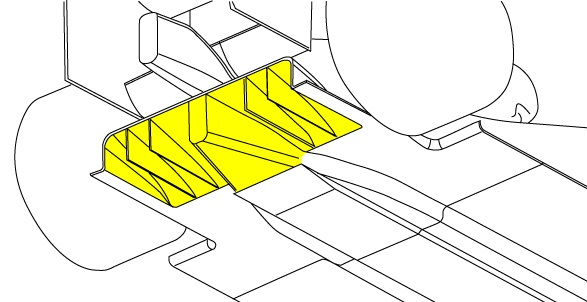
\includegraphics[scale=0.6]{Figures/diffuser_fences.jpg}
  \end{subfigure}
  %
  \begin{subfigure}[b]{0.4\textwidth}
    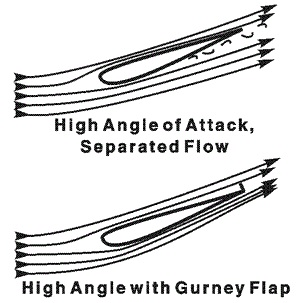
\includegraphics[scale=0.8]{Figures/Gurney.jpg}
  \end{subfigure}
%  
  \caption{Fences or strake on a diffuser(left) and example of a Gurney flap application on a wing (right) \cite{Anonymous2020GurneyFlap}.}
    \label{fig:gurney}
\end{center}
\end{figure}

\noindent Fence or strake on a diffuser acts as a force generator. As discussed previously, the corner vortices at the rear diffuser generate downforce, and strake helps the diffuser generate more vortices, increasing more downforce. Figure \ref{fig:gurney} left shows the example of a basic strake on a diffuser. Gurney flap is a small flap or L-shape structure attached at the end of the diffuser, shown in figure \ref{fig:gurney} right. Generally, the Gurney flap is used to improve downforce without significant drag \cite{Willemsen2012CFD-basedDiffuser} by making the boundary layer stay attached and delay flow separation to the end of the diffuser by reducing the pressure on the underside of the diffuser and increasing the pressure on the top of the diffuser. 

\noindent Despite the advantageous function of both devices, Undertray research is still a privilege in the racing industry which create a significant information gap in this industry. Therefore, further analysis in this field will be a good leap in improving undertray performance.  
